\documentclass[a4paper, amsfonts, amssymb, amsmath, reprint, showkeys, nofootinbib, twoside]{revtex4-1}
\usepackage[spanish]{babel}
\usepackage[utf8]{inputenc}
\usepackage{float}
\usepackage[colorinlistoftodos, color=green!40, prependcaption]{todonotes}
\usepackage{amsthm}
\usepackage{mathtools}
\usepackage{physics}
\usepackage{xcolor}
\usepackage{graphicx}
\usepackage[left=23mm,right=13mm,top=35mm,columnsep=15pt]{geometry} 
\usepackage{adjustbox}
\usepackage{placeins}
\usepackage[T1]{fontenc}
\usepackage{lipsum}
\usepackage{csquotes}
\usepackage[normalem]{ulem}
\useunder{\uline}{\ul}{}
\usepackage[pdftex, pdftitle={Article}, pdfauthor={Author}]{hyperref} % For hyperlinks in the PDF
%\setlength{\marginparwidth}{2.5cm}
\bibliographystyle{apsrev4-1}

\begin{document}

%El título del experimento realizado es importante.
\title{Carga-Masa (Antiguo)}


\author{Sergio Montoya Ramirez}
\email[Correo institucional: ]{s.montoyar2@uniandes.edu.co}

%Si necesitan poner un segundo autor, deben eliminar los porcentajes (%) iniciales.
  
%\author{Second Author}
%\email{Second.Author@institution.edu}

\affiliation{Universidad de los Andes, Bogotá, Colombia.}

\date{\today} % Si lo dejan vacío no les saldrá fecha. La fecha que se muestra es del día en que se compila.

\begin{abstract}

En este se describen brevemente los objetivos y los resultados del trabajo, por lo tanto se debe dar información completa pero corta del contenido del trabajo. Se debe indicar qué fue lo que se hizo, cómo se hizo y cuáles fueron los resultados obtenidos.

\end{abstract}

\maketitle

\section{Introducción}

Durante el nacimiento de la mecánica cuántica a principios del siglo $XX$ el mundo científico se encontraba deseoso de entender mas esta rama. Por lo tanto, era prioritario para esto medirlo. Deseábamos saber de manera exacta la mayor cantidad de variables que fuera posible de cada partícula. En medio de todo este desarrollo se encontraba el electrón. Una de las partículas primordiales para los átomos y para el entendimiento de la mecánica cuántica. El electrón reunía muchas características cuánticas que sorprendían a aquellos que lo estudiaban. Una de estas características es la gran dificultad (quizás imposibilidad) de medir su masa o carga. Sin embargo, el físico J.J. Thomson encontró una manera de medir la relación que estas dos magnitudes tenían entre si. Para conseguir esto, Thomson lanzo electrones a una pantalla a través de un campo magnético generado por una bobina de Helmholtz. Sin embargo, nosotros el día de hoy haremos un experimento equivalente mas no análogo. En este experimento, el campo sera generado por un Solenoide y por lo tanto para nuestro caso la relación carga masa seria
\begin{equation}
  \label{eq:CargaMasa}
  \frac{e}{m}=\frac{8\pi^2}{\mu_0^2}\frac{n^2}{N^2}\frac{L^2}{l^2}\frac{V^2}{I^2}
\end{equation}

Donde $\mu_0$ es la permeabilidad magnética del espacio libre. $N$ es el numero de vueltas que tiene el solenoide. $n$ es el numero de hélices que describe el electrón.  $L$ es la longitud de la bobina.  $l$ es la longitud del tubo de rayos catódicos y  $v$ es el voltaje.
\section{Montaje experimental}

\begin{figure}[h]
    \centering
    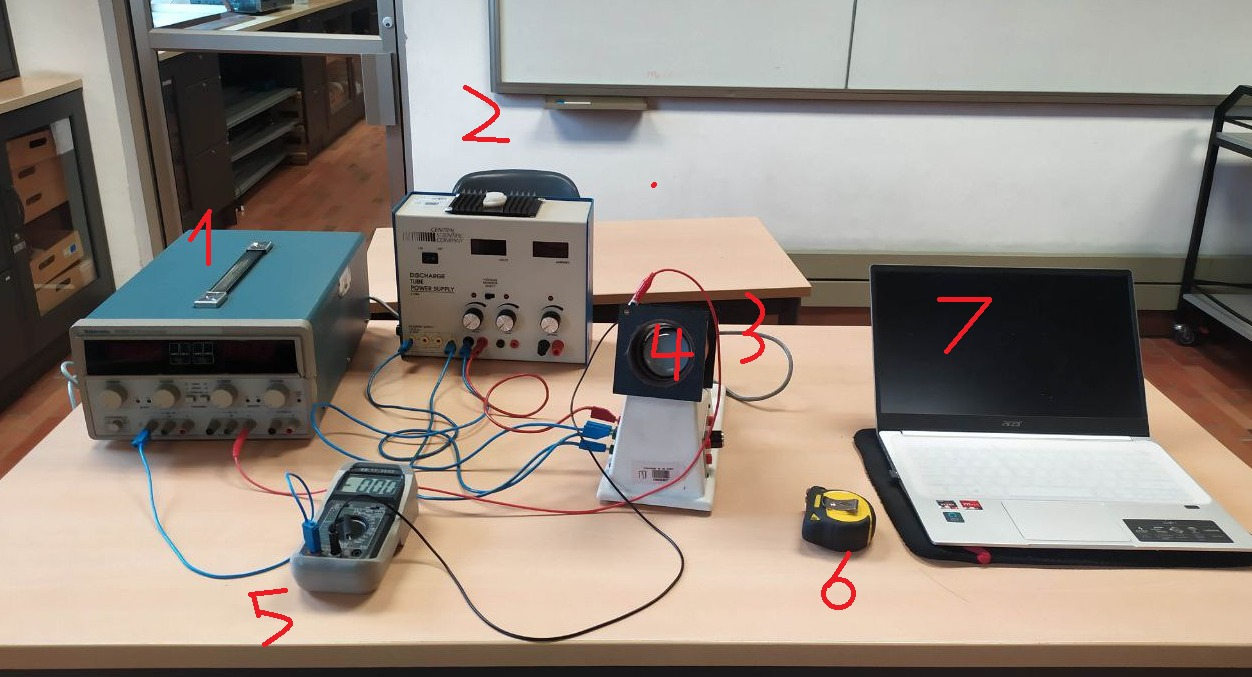
\includegraphics[width=8cm]{cma_montaje_marcado.jpeg}
    \caption{Fuente de corriente (1), fuente de voltaje (2), bobina (3), tubo de rayos catódicos (4), multímetro (5), cinta métrica (6) y computadora (7).   }
    \label{fig:MontajeG}
\end{figure}

Lo primero que hacemos es conectar el tubo de rayos catódicos con su fuente de voltaje y la bobina a una fuente de corriente. Después de esto, Fijamos varios valores de voltaje de disparo de tal manera que todos produzcan un rayo visible. Luego, para cada uno de estos valores de voltaje buscamos varios valores de corriente que enfoquen nítidamente el rayo de electrones. Con esto se muestra que el electrón tuvo un numero entero de hélices. Para saber el numero exacto de vueltas dadas se puede contar desde el caso en el que no hay campo (es decir sin corriente) sabiendo que en ese caso hay también 0 hélices.

\section{Resultados y análisis}

De los datos obtenidos se realizaron cuatro distintas regresiones lineales. Una por cada grupo de voltaje contra corriente. Sin embargo, la regresión se hizo en función de $V$ y  $I^2$, De ellas se encontró la pendiente intercepto y el error. Los datos se encuentran en la tabla \ref{tab:Pend}
 \begin{table}[htpb]
  \centering
  \caption{Tabla de datos de las regresiones lineales en función de $V$ y  $I^2$}
  \label{tab:Pend}
  \begin{tabular}{|c|c|c|}
    \hline
  $n$ & $m\left( \frac{V}{A^2} \right) $ & error \\
  \hline
  1 & 328.99 & 6.96 \\
  2 & 89.80 & 12.23 \\
  3 & 44.13 & 5.09 \\
  5 & 28.63 & 7.86 \\
  \hline
  \end{tabular}
\end{table}

Luego de esto tomamos la ecuación \ref{eq:CargaMasa} y la reescribimos para que nos quede como sigue \[
V = \frac{\mu_0^2}{8\pi^2}\frac{N^2 l^2 e}{n^2 L^2 m}I^2
.\] Dada la regresión que tenemos sabemos que el termino que acompaña a $I^2$ es la pendiente que denominaremos $p$ para evitar confusiones con la masa. Por lo tanto despejando para  $\frac{e}{m}$ nos queda \[
\frac{e}{m}=p \frac{8\pi^2}{\mu_0^2}\frac{n^2}{N^2}\frac{L^2}{l^2}
.\] Luego de esto y aprovechando cada una de las pendientes obtenidas previamente podemos obtener la tabla \ref{tab:em}
\begin{table}[htpb]
  \centering
  \caption{Tabla de la relación carga masa para el electrón obtenida por medio de los datos de la tabla \ref{tab:Pend} y la ecuación \ref{eq:CargaMasa}}
  \label{tab:label}
  \begin{tabular}{|c|c|c|}
    \hline
    $N$ &  $\frac{e}{m}$ & error \\
    1 & $3.972\times 10^{10}$ & 6.96 \\
    2 & $4.337\times 10^{10}$ & 12.23 \\
    3 & $4.975\times 10^{10}$ & 5.09 \\
    4 & $5.530\times 10^{10}$ & 7.86\\
  \end{tabular}
\end{table}
Si realizamos el promedio de estos valores el resultado termina siendo un orden de magnitud inferior con lo esperado por la teoría. Esto puede ser ocasionado pues a la hora de tomar los datos se presento una muy baja precisión. Entre los errores presentes a la hora de realizar la toma de datos se encontraba un error sistemático de la fuente de voltaje (que tenia una variación de aproximadamente una unidad). Ademas de el hecho de que nunca se registraba un campo nulo (Incluso cuando se marcaba la fuente de corriente a 0) cosa que se evidenciaba pues en esta circunstancia había cierto esparcimiento en la pantalla en vez de un punto como se esperaba.

\section{Conclusiones}

Se deben contestar las preguntas planteadas inicialmente o dar las razones por las cuales no es posible hacerlo. Las conclusiones deben ser necesariamente una consecuencia del experimento realizado, es  decir  que  no  se  deben  tocar  aspectos  que  no  se  hayan  expuesto  en  la  sección  de resultados y análisis. Si escribe algo que no se encuentra en la sección de resultados y análisis,  esto quiere decir que hace falta incluir material en resultados y análisis. Concluir únicamente aspectos pertinentes al trabajo obtenido en el laboratorio; se deben evitar las generalizaciones que no hablan concretamente de lo que lograron o midieron en la práctica experimental. 



\bibliographystyle{abbrv}
\bibliography{Referencias}
\nocite{Ejemplo}

\section*{Apéndice de cálculo de errores}

Se deben indicar explícitamente los pasos de análisis de error que se hicieron para llegar a al(los) resultado(s). Ejemplo: la propagación de error, incertidumbre en un ajuste de mínimos cuadrados, análisis estadístico, redondeo de cifras significativas, entre otros.

Las fórmulas de cómo se obtuvieron cada uno de los valores reportados debe ser incluido como si análisis estadístico se hiciera manualmente.
\end{document}
